\documentclass{mcmthesis}
  \mcmsetup{CTeX = false,   % 使用 CTeX 套装时,设置为 true
          tcn = 88022, problem = B,
          sheet = true, titleinsheet = true, keywordsinsheet = true,
          titlepage = false, abstract = true}
  \usepackage[english]{babel}
  \usepackage{fontspec}
  \usepackage{palatino}
  \usepackage{lipsum}
  \title {PEIL: a Novel Prediction Model for Language Geographic Distribution on Time Series}
  \date{}
  
  \setmainfont{Times New Roman}
  \begin{document}
  \begin{abstract}
  
    %\indent With the development of globalization, people get to know more about other tongues, so the research about the language rises. Recently, a multinational service company wants to expand to be more international and have employees who can speak different several languages. For this sake it needs to know the trends of global languages and wants to get advice about new offices's locations.\\
    \indent This paper establishes three major models to address both geographic distribution and time variation of global languages. By mining related data, we adopt our novel models on the prediction of languages across the world, thus providing the best recommendations on the selection of new offices for a multinational company.\\
    \indent Firstly, in order to get a high-level idea of the overall trends, we mine big data from packaged datasets, web pages and an enormous sampled Twitter corpus of 48h. Secondly, we build a proper model to capture the changing pattern of nations' major eco-social statistics on time series, which is later used to make predictions on required information in 50 years. Thirdly, we select typical fields and study the dependency relationship between population, exports, imports and language use, which we conclude as a novel model to connect geographic distribution with time variation. Lastly, we cluster the data from social media, which suggests the multi-language use of world population, helping us with the decision making in practice.\\
    \indent During our research, we make full use of available resources. In the process of building and optimizing models, we give reasonable analysis, explanation, and validation. In this paper, we also discuss the pros \& cons of our models, as well as future work.\\
    
  \begin{keywords}
    language map prediction, time series model, K-means clustering, siting problem
  \end{keywords}
  \end{abstract}
  \maketitle
  \pagestyle{empty}
  \newpage
  \tableofcontents
  \setmainfont{Times New Roman}
  \newpage
  \pagestyle{fancy}
  \setcounter{page}{1}
  \section{Introduction}
  \subsection{Background}
    \indent \indent Half of the world's population speak one of ten languages as their native language, although there are nearly 7,000 languages spoken on the earth. But with the influence of government, culture, economy and the impact of globalization, popularity of each language varies over the time. As an important part of human civilization, researches related to languages stay heated all the time. Many researchers and research institutes did surveys on languages of the world such as the Ethnologue website. Besides, international companies which are willing to expand global business also put some attention on languages study because languages are a powerful tool for them to connect the world and create a global market. \\
    \indent So a Chief Operating Officer of a multinational service company wants to know the trends of global languages, including the variation of total number of speakers and the geographic distribution of particular language. Based on these results he or she also wants to know locations for this company's new international offices. So we implemented a PEIL model to predict the trends and used K-means algorithm to help this company make the choice.
  \subsection{Restatement of the Problem}
    \indent \indent First of all, we are required to build a model to predict the trends of global languages, considering the influence from multiple factors. The trends of languages include the changes in the number of total speakers using a particular language, which can be divided into native speakers and non-native speakers. 
    
    \indent After that, using the trends we predict, we should then tell variation of the top-10 languages lists. And we are also required to study the geographic distribution change of all languages. Then we need to decide where the new international offices of the company should be located, and try to take efforts to reduce the number of offices considering the changing nature of global environment and the necessity of saving resources.
   \subsection{Our work}
    \begin{itemize}
      \item We proposed a novel model based on classical gravity model, considering the influence that one language gets from the world as an effect which is similar to gravity.
      \item We used the well-known ARIMA model to help us get the intuition of data variation. We analyzed the factors that might influence the variation of languages and made simple predictions on these factors.
      \item We used the K-means algorithm to identify the locations of new international offices of this company and combined the elbow method to determine the best number of new international offices.
    \end{itemize}
  
  % \emph{center of percussion} [Brody 1986], \lipsum[5]
  
  % \begin{Theorem} \label{thm:latex}
  % \LaTeX
  % \end{Theorem}
  % \begin{Lemma} \label{thm:tex}
  % \TeX .
  % \end{Lemma}
  % \begin{proof}
  % The proof of theorem.
  % \end{proof}
  
  \section{Basic Assumptions}
  \subsection{Assumption 1.}
  
    \indent \indent We assume that the static factors of every country doesn't change during the period of time we study. These factors include the GDP, land area, geographic position and so on.
  
  
  \subsection{Assumption 2.}
  
    \indent \indent We ignore unpredictable or low-probability events that may cause great impact to languages trends.
    
  \subsection{Assumption 3.}
  
    \indent \indent We ignore internal effects of the selected target group, only consider the inner-outer interaction.
   
  % \begin{figure}[h]
  % \small
  % \centering
  % 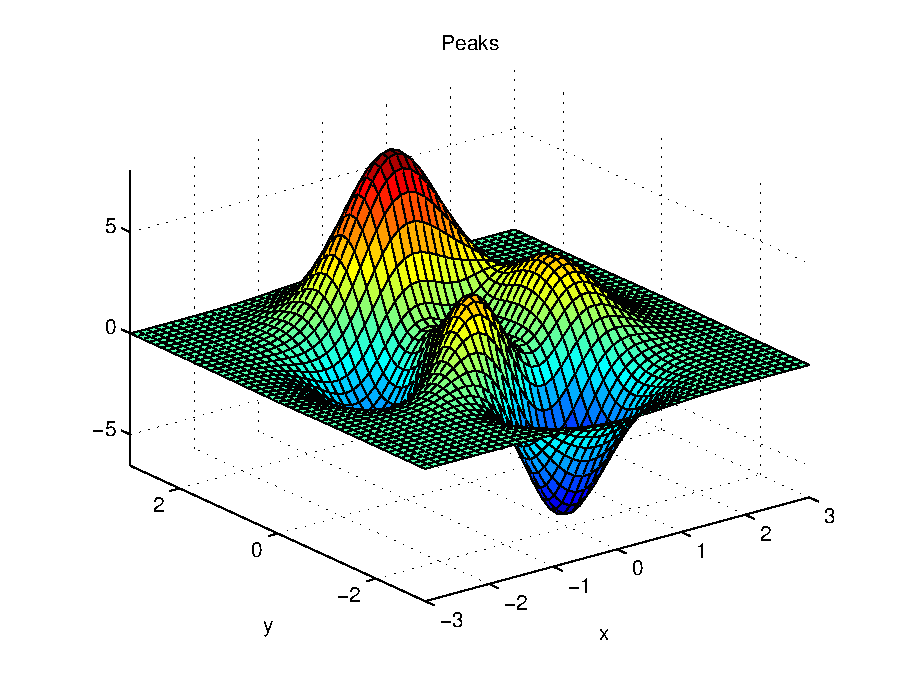
\includegraphics[width=12cm]{mcmthesis-aaa.eps}
  % \caption{aa} \label{fig:aa}
  % \end{figure}
  
  % \lipsum[8] %\eqref{aa}
  % \begin{equation}
  % a^2 \label{aa}
  % \end{equation}
  
  % \begin{equation}
  % e^{i \theta} = \cos \theta + i \sin \theta \label{bb}
  % \end{equation}
  
  % \[
  %   \begin{pmatrix}{*{20}c}
  %   {a_{11} } & {a_{12} } & {a_{13} }  \\
  %   {a_{21} } & {a_{22} } & {a_{23} }  \\
  %   {a_{31} } & {a_{32} } & {a_{33} }  \\
  %   \end{pmatrix}
  %   = \frac{{Opposite}}{{Hypotenuse}}\cos ^{ - 1} \theta \arcsin \theta \eqno(3)
  % \]
  
  % \lipsum[9]
  
  % \[
  %   p_{j}=\begin{cases} 
  %   0,&\text{if $j$ is odd}\\
  %   r!\,(-1)^{j/2},&\text{if $j$ is even}
  %   \end{cases}
  % \]
  
  % \lipsum[10]
  
  % \[
  %   \arcsin \theta  =
  %   \mathop{{\int\!\!\!\!\!\int\!\!\!\!\!\int}\mkern-31.2mu
  %   \bigodot}\limits_\varphi
  %   {\mathop {\lim }\limits_{x \to \infty } \frac{{n!}}{{r!\left( {n - r}
  %   \right)!}}} \eqno (1)
  % \]
  
  \section{Models and Methodology}
    \subsection{Time Series Prediction}
    \indent \indent In order to have an intuition about how the factors that have influence on languages will change in the next 50 years, we use the well-known ARIMA model to predict them. ARIMA model, i.e autoregressive integrated moving average model, is a widely used method for predicting time series. Considering these factors change over the time, and in order to simplify this problem, we regard them as factors only related to time. The ARIMA model can be represented as following formula.
  
    \begin{equation}
      \left(1-\sum^p_{i=1}\sigma_i L^i\right)(1-L)^d X_t = \left(1+\sum^q_{i=1}\theta_i L^i\right)\epsilon_t
    \end{equation}
  
    \indent In the equation above, $L$ stands for Lag Operator, d$\in$Z, d$>$0.
  
    \indent Considering these factors we use vary randomly and are related to many other factors, they are not stationary variables and can not be directly used int ARIMA model. So we calculate the difference of factors we study and apply ARIMA model on them. After getting the forecast result we calculate the accumulation to restore prediction result. Take the GDP prediction for an example, we collect the GDP of countries from 2002 to 2016, calculate the difference of adjacent years and use the $ARIMA$ model of $Python$ language. After this ARIMA model gives us the prediction of how the difference of a country's GDP will change in the next 50 years, we calculate the accumulation of this prediction values and regard the final sum as our prediction on this country's GDP.
    
    \indent The results we got from time series prediction show us the approximate trends about how these factors will change during the next 50 years. But limited by the amount of data we collected, it's not reasonable to predict a long term process with only a few data points. So we finally used the following PEIL model for a better prediction.
  
  
  \subsection{The PEIL Model}
  \indent \indent Based on external knowledge we acquired via Assumption 3 and inspired by the structure of the classic Gravity Model, we  develop a novel Population-Export-Import-Language(PEIL) model to address the geographic distribution of language use. Specially, we focus on the major/official language family per nation to achieve better conciseness.
  \indent Given the obvious interdependency between a nation's international eco-social status and its language use, and based on Assumption 3, we first model the dynamics of global language intervention with economic interaction. To better describe the degree of such intervene, we inspect exports and imports stats, as they are reflections on both economy and openness factors. As volume vary from nation to nation, we pay attention on qualifying the weights different languages makes in a nation's economic growth, thus utilizing ${D_{export}}$ and ${D_{import}}$ in the formula(2) to depict the degree of external influence on language $l$ respectively.
  
  
  
  \begin{equation}
  \begin{aligned}
  {D_{export}}_{(l)}=\sum_{i}{P_{l}}_{(i)} \cdot S_{export}/S_{GDP}\\
  {D_{import}}_{(l)}=\sum_{j}{P_{l}}_{(j)} \cdot S_{import}/S_{GDP}
  \end{aligned}
  \end{equation}
  
  \indent i and j are the descending ranks of percentage $P_{l}$ in net exports $S_{export}$ and net imports $S_{import}$, while $S_{GDP}$ represents the Gross Domestic Product in the same periods. In our implement, we investigate our study targets' major commercial partners to represent such bias.
  
  \indent In analyzing the graphs, we discover that in most cases, the larger population volume is, the more stable language structure will be. It's an phenomena with high interpretability, since under external influence at the same degree, great population will postpone the development of the resulting trend. Interestingly, this nature of "stubbornness" shares similarity with inertia in classic physics. However, the inverse-square pattern doesn't apply to the rough value of population $S_{population}$ versus language structure change. Instead, we observe an obvious inversely proportional relationship. Therefore, we can calculate the instant growth rate of the speakers percentage $Y_{l}$ with the equation:  
  
  $$Y_{l}=f({D_{export}},{D_{import}}_{(l)})/S_{population}$$
  
  \indent To acquire the needed data, we turn to CIA's World Factbook[2], which provides us with great rich information on various eco-social stats. As for the specified implement of binary function $f(x_{1},x_{2})$, We first retrieve the related data via corresponding fields in HTML documents with defined filters, then we discuss coordients which have symmetrical structures, since export and import map to a stat pair in reality. To the best of our knowledge, a sum function works best. Then we conclude the PEIL model in the equation.
  
  $$Y_{l}=(\alpha \cdot {D_{export}}+ \beta ]\cdot {D_{import}}_{(l)})/S_{population} + \gamma$$
  \indent Given the Time Series Prediction model discussed in 4.1, it's practical to make a relatively accurate prediction on future GDPs, exports and imports. However, as we fail to fully collect the business partnership for all nations, we are unable to precisely draw a high-level picture of the future global language distribution. However, investigation on the development of World's major languages offers a promising stability, suggesting that we can directly infer the reasonably-near future from the perspective nowadays. Furthermore, given population-related changes, the model will automatically makes adjustments by selecting the new population as its input. 
  \indent The training set comes from CIA's World Factbook. After trained on the available datasets, we take $\alpha=0.202017$,$\beta=0.957035$,$\gamma=0.097274$ as the best parameters. As for the validation of our PEIL Model, we construct experiments on test sets, which is detailedly stated and illustrated in 5.1.
    \subsection{K-Means}
  
    \subsubsection{New Offices}
  
    \indent \indent In order to get the best locations for this company's six new offices, we resort to the power of social network. Concretely, we use data sampled in Twitter for 24 hours, which we think can represent the one day's social life of people around the world well. The data sampled from Twitter API gives us the information about the locations of twitter users[6], the language of tweets and the origin language of users when he or she registered Twitter. 
  
    \indent Considering this company is a multinational service company and needs to be more international, its new offices should be close to its clients or potential customers. In densely populated areas, there is a higher possibility that more people can be the potential customers of the company. As we know, nowadays more and more people are using social software to keep track of life, for example twitter, facebook, ins etc. So these software contents are a useful means to analyze the population distribution, especially posts with position information. So we mark the locations of twitters on a world map and use K-means algorithm to find centroids of different clusters of twitters. Obviously, these centroids are centers of crowd and offer great opportunities for companies.
    
    \indent Because of the need for multi-language speakers of this company, it is important to consider the language environment of these new offices. To simplify this problem, we regard the users whose twitters use a different language from his or her registration language as a potential polyglot, so the language environment around them might be more open and attractive. Based on this assumption we pick those "polyglots" from our data and apply K-means algorithm on them. After setting $K$ to be equal to 8 (This company already has two offices in Shanghai and New York, so the total number of offices will be 8), we got the following results, as show in Figure 1. 
  
    \begin{figure}[h]
      \small
      \centering
      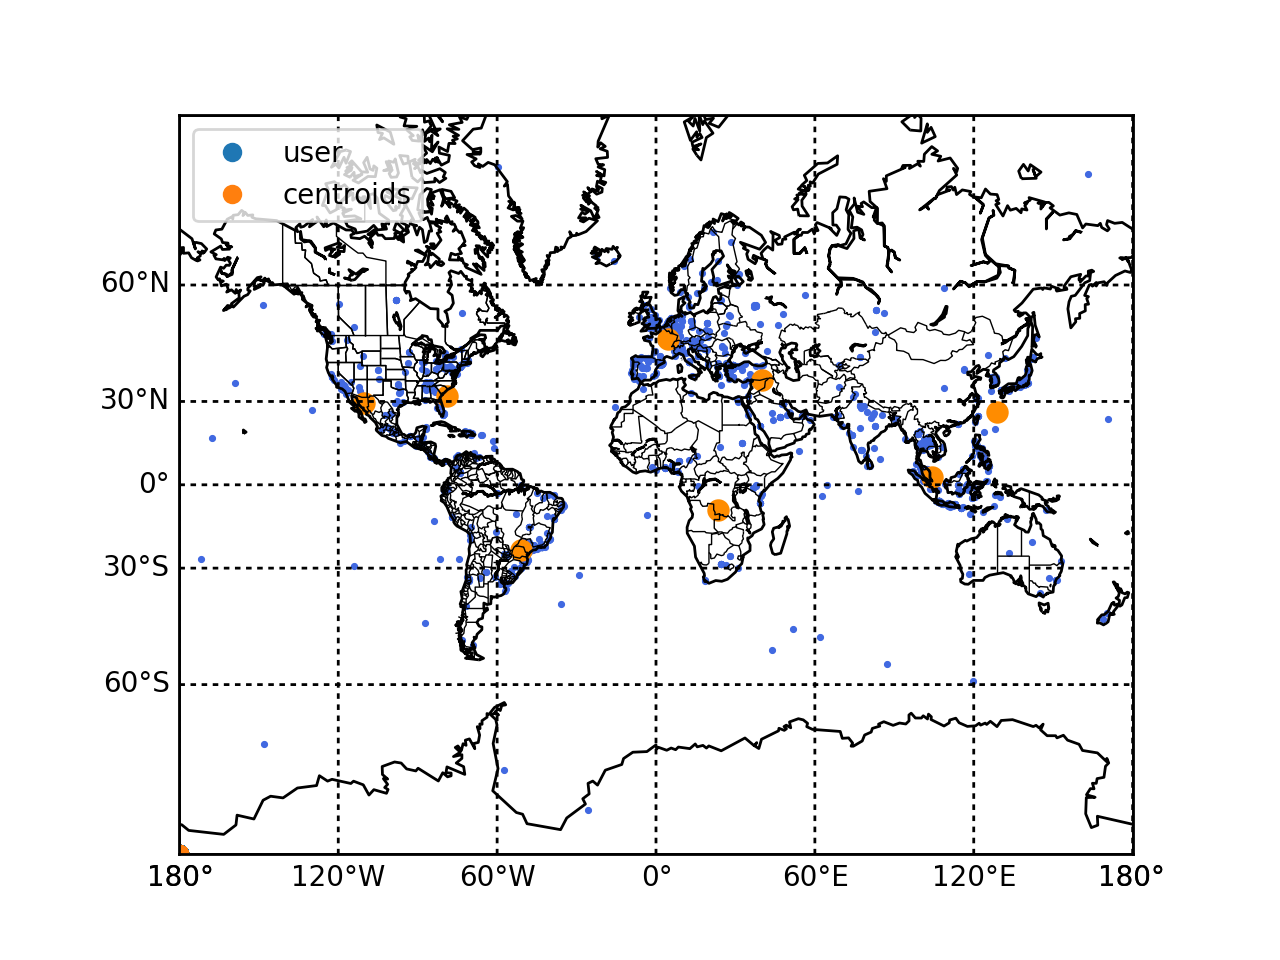
\includegraphics[width=12cm]{world_offices.png}
      \caption{New offices' distribution} 
    \end{figure}
    \newpage
  
    \indent Our result shows all eight locations that is appropriate to set up new offices. Apart from the two offices that already exist in Shanghai and New York (which may not be exactly on its true place on this map, but in consideration of sampling errors, we think it is still reasonable to regard the points lies on east coast of North America and China to be New York and Shanghai), we can still see the other six new offices. They are located in San Francisco, São Paulo, Paris, Jerusalem, Kinshasa and Singapore. It is shown that they are nearly located in separated continents on earth, which is in accordance with the need to get a more open language environment.
  
    \indent In terms of what languages will be spoken in these six new offices, we still use the data from Twitter to help us decide. We collect twitter users that are near the six new offices and count the types of languages of these tweets. Let us use the office in Paris as an example, we calculate what types of languages are used by twitter users around Paris and how many tweets are sent using corresponding language. The result can be shown as follows. Figure2 shows the number of twitter users with different languages around the office located in Paris.
  
    \begin{figure}[h]
      \small
      \centering
      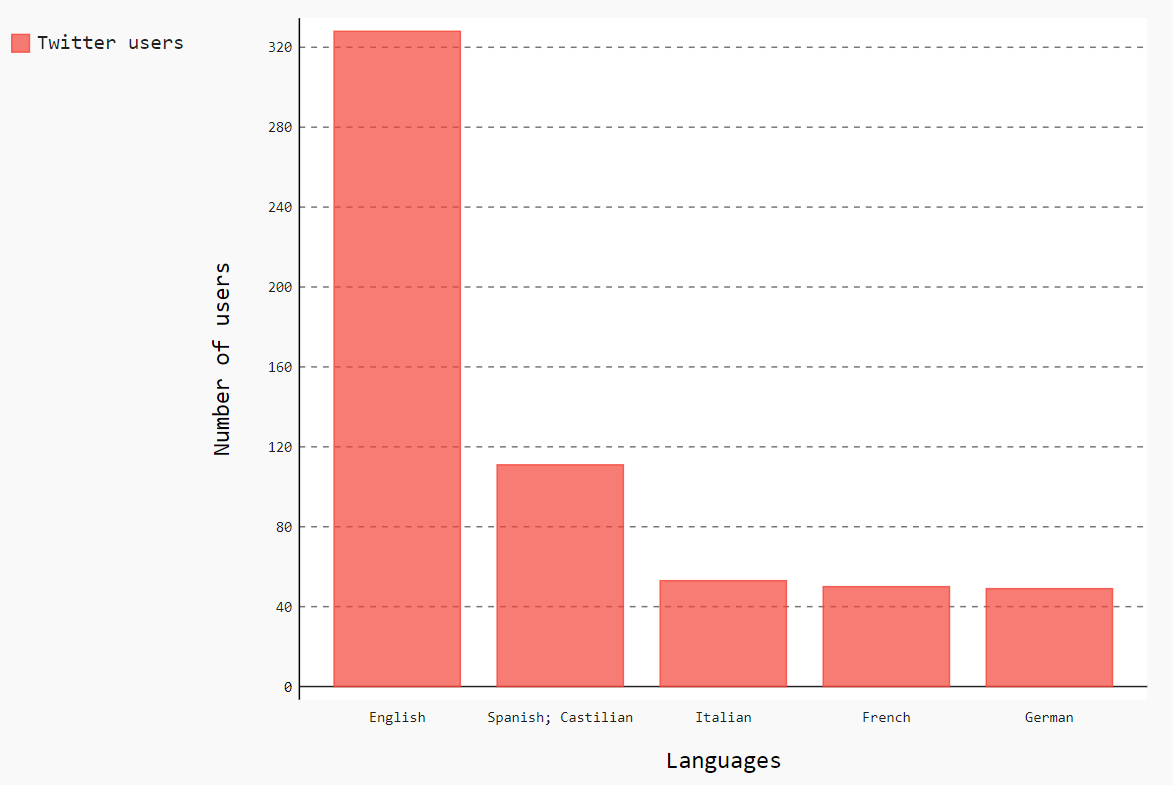
\includegraphics[width=10cm]{paris.png}
      \caption{Languages spoken in Paris}
    \end{figure}
    \newpage
  
    \indent So languages spoken in the office in Paris might be English, Spanish, Italian, French and German. And here are the languages spoken in other new offices.
    \begin{itemize}
      \item Office in San Francisco: English, Spanish, French, Japanese and Portuguese.
      \item Office in São Paulo: Portuguese, Spanish, English, Japanese and Finnish.
      \item Office in Jerusalem: Turkish, English, Russian, Arabic and Japanese.
      \item Office in Kinshasa: English, Spanish, French, Portuguese and Afrikaans.
      \item Office in Singapore: Chinese Mandarin, English, Indonesian, Thai and Spanish.
    \end{itemize} 
  
    \indent The K-means model we use is from $Python$. It uses an effective k-means++ algorithm to speed up the total clustering process. The intuition of k-means++ algorithm can be interpreted as follows: when choosing the next centroid, we always select the centroid that is far from all centroids that have already been chosen. This meets with the desire to be more international because it disperses the new offices and make them distributed globally. 
  
    \subsubsection{Less Offices}
  
    \indent \indent The K-means model can also help us identify the best number of new offices. We transform the problem into finding best number of clusters in a data set. Here we use the elbow method, which is a convenient but also efficient way to find the best K in K-means algorithm. The key index of this method is SSE(sum of squared errors), which is defined as follows:
    \begin{equation}
      \mathop{SSE} = \sum^k_{i=1}\sum_{p\in C_i}\left|p-m_i\right|^2
    \end{equation}
    \indent Where $k$ stands for the number of clusters and $m_i$ denotes the centroid of cluster $i$, so $p$ is the point in cluster $i$. The elbow method tells us that generally when the number of clusters increases, the SSE of whole model will descend rapidly at first but slow down soon afterwards. So an "elbow" point will appear and it corresponds to the best number of clusters that the K-means algorithm should choose. Here is the elbow method result for this problem.
  
    \begin{figure}[h]
      \small
      \centering
      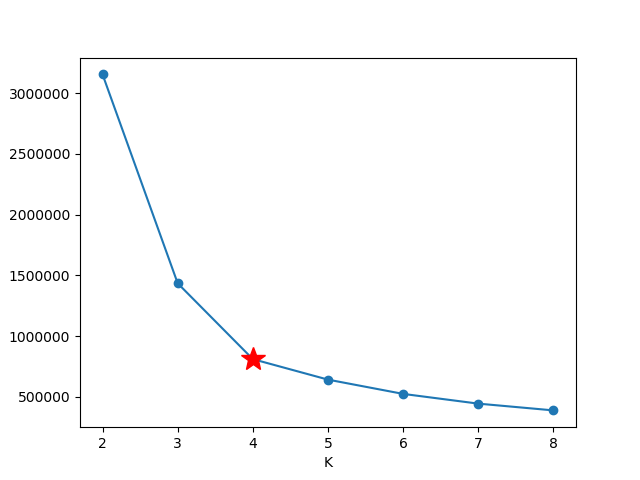
\includegraphics[width=12cm]{elbow_method.png}
      \caption{Results of elbow method}
    \end{figure}
    \newpage
  
    \indent According to this result, this company should open two more international offices, as the best number of clusters should be four. And after using the K-means algorithm above we got the result that the two new international offices should be located in Paris and São Paulo.
    
  \section{Validating the Model}
  \indent\indent Among all the nations that have detailed data of commercial bias, we choose the following seven rows: English in Canada(2000-2006); English in New Zealand(2000-2011); Chinese in Singapore(2006-2012); English, French, German and Italian in Switzerland. The prepared dataset before fed into our PEIL Model in listed as follows. 
  
  %%%%%%%%%% TABLE OBJECT %%%%%%%%%%
  \begin{table}[!htbp]
  \centering
  \begin{tabular}{lrrrr}
  \multicolumn{1}{c}{NATION\_LANG}&\multicolumn{1}{r}{LANG\_RATE}&\multicolumn{1}{r}{EXPORT\_RATE}&\multicolumn{1}{r}{IMPORT\_RATE}&\multicolumn{1}{r}{POPULATION}\\
  \multicolumn{1}{c}{CAN\_EN}&\multicolumn{1}{r}{$-0.083$}&\multicolumn{1}{r}{$-0.559585763$}&\multicolumn{1}{r}{$-1.189910524$}&\multicolumn{1}{r}{$33.759742$}\\
  \multicolumn{1}{c}{NZL\_EN}&\multicolumn{1}{r}{$-0.2$}&\multicolumn{1}{r}{$0.268073902$}&\multicolumn{1}{r}{$-0.182007664$}&\multicolumn{1}{r}{$0.425277$}\\
  \multicolumn{1}{c}{SGP\_ZH}&\multicolumn{1}{r}{$0.13$}&\multicolumn{1}{r}{$0.250799792$}&\multicolumn{1}{r}{$-0.255541048$}&\multicolumn{1}{r}{$4.701069$}\\
  \multicolumn{1}{c}{SWE\_EN}&\multicolumn{1}{r}{$0.3$}&\multicolumn{1}{r}{$0.519949311$}&\multicolumn{1}{r}{$0.36181698$}&\multicolumn{1}{r}{$7.623438$}\\
  \multicolumn{1}{c}{SWE\_FR}&\multicolumn{1}{r}{$0.183$}&\multicolumn{1}{r}{$0.197373888$}&\multicolumn{1}{r}{$0.160014223$}&\multicolumn{1}{r}{$7.623438$}\\
  \multicolumn{1}{c}{SWE\_DE}&\multicolumn{1}{r}{$0.1$}&\multicolumn{1}{r}{$0.501031609$}&\multicolumn{1}{r}{$0.942099583$}&\multicolumn{1}{r}{$7.623438$}\\
  \multicolumn{1}{c}{SWE\_IT}&\multicolumn{1}{r}{$0.15$}&\multicolumn{1}{r}{$0.211092615$}&\multicolumn{1}{r}{$0.302645088$}&\multicolumn{1}{r}{$7.623438$}\\
  \end{tabular}
  \caption{Test data}
  %\label{tab:}
  \end{table}
  
  \indent In order to better address the effectiveness of this model, we make a validation experiment on EViews 6.0 (win10 pro x64, EID=16299.214). We take the last three columns as input, and get the returning value as output. Then, we plot the fitted, actual increment rates, together with their residual. As shown in Figure 4, it produces a result beyond satisfactory. 
  
    \begin{figure}[h]
      \small
      \centering
      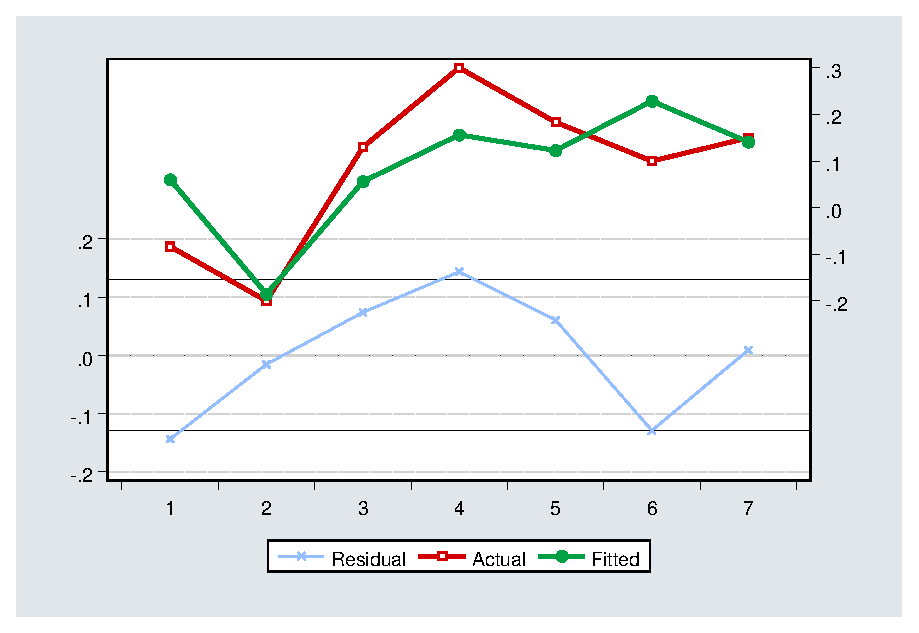
\includegraphics[width=12cm]{valid_peil.eps}
      \caption{Actual, fitted, residual graph}
    \end{figure}
    \newpage
  
  \section{Conclusions}
  \subsection{Prediction on language use in 50 years}
  
  \indent \indent By analyzing the related statistics vary from year to year, we conclude that the percentage of each major language shows stability. The structure of PEIL Model also reveals that. This phenomenon is basically for the contribution of first speakers. The first/official language(s) of a given nation are very likely to remain still in the predictable time period. Thus, the percentage of native(L1) speakers of major languages won't have a huge difference in 50 years. And because native speakers make up the majority of the speakers groups, the global structure of total language speakers will develops stably as well. 
  
   \indent As for the L2 speakers, we can predict their amount by simply rid the L2 speakers' amounts from the total ones.
  
  \subsection{Conclusions for geographic distributions change over time}
  
  \indent Since at present we haven't collect enough data, it's hard for us to directly model the global distributions. However, we have validated  our methodologies on various languages in various nations. With more information of bias on exports and imports per nation, we can approximate the accurate prediction.
  
  \indent Furthermore, given the global population and human migration patterns, we are enabled to predict the population change overtime in different nations, which will then makes adjustments to the final input of population factor to our model. In other word, this update can increase the accuracy of our prediction.  
  
  \subsection{Conclusions for new offices}
  \indent \indent We recommend the six new offices of this company to be located in are San Francisco, São Paulo, Paris, Jerusalem, Kinshasa and Singapore. Based on our assumptions above, these cities are centroids of open and vigorous environment, which means they are great places for this company to develop business. And with the languages each office might speak listed above, we can summarize that English, Chinese Mandarin, Spanish, French, Turkish and Portuguese might be the most common languages of these offices.
  
  \indent Besides, using the elbow method above, we found that it might be better for this company to open just two new offices because this plan saves more resources and covers considerable amount of clients of the world. And using the K-means algorithm again we found that the two new offices should be located in Paris and São Paulo. 
  
  
  \section{Strengths and weaknesses}
  
  \subsection{Strengths}
  \begin{itemize}
  \item \textbf{Promising prediction ability }\\
    As reviewed in Part 5, our PEIL Model work out well on validation datasets. Since given enough information, we can make relatively accurate prediction on major time series statistics, our prediction models have promising ability and feasibility.
   \item \textbf{Reality oriented}\\
    We climb big data from Twitter Stream, which turns out to be a novel idea on collecting real-time data. What's more, this method shows bias on the area where people are better involved with modern technology and life style, which is important and helpful in our target decision-making problem.
    \item \textbf{Self-adaption character}\\
    The overall architecture of our models can be summarized as two parts, the time variation department and the geographic distribution department. Before connected to each other by PEIL Model, they function independently, which minimizes the spread of error and maximizes the flexibility.
  \end{itemize}
  \subsection{Weaknesses}
  \begin{itemize}
     \item \textbf{Long-term predictions by K-means can't be made }\\
    The data we collected from Twitter is only one day's data. So we can use it to make short-term predictions. But the long-term prediction with K-means algorithm lacks the necessary statistics so its result in long term is not particularly convincing. As a matter of fact, we have noticed such info via web, but owing to time limit, we are unable to collect them.
  
    \item {\textbf{Some other factors may affect} }\\ 																In our model, we choose some typical factors to analyze. However, there are some other factors that could make influences to language development, such as religions, age structures, sex ratio, ethnic groups etc.
  \end{itemize}
  
  
  \section{Memo}
  
  \textbf{To}: Chief Operating Officer of the service company\\
  \textbf{From}: MCM Team Members\\
  \textbf{Subject}: Results and Recommendations\\
  \textbf{Date}: {\today}\\
   \noindent\rule{\textwidth}{0.5pt}
   
      Languages play a more and more important role in our life, it makes sense to analyze the speakers distribution of languages and predict the changes in the future. However, the fact that there are nearly 7,000 languages spoken on the earth and diversity of languages within a nation makes the work difficult. We established the mathematical models to simplify the actual problem, thus making a prediction and drawing a conclusion.
      
     \indent We take many factors into consideration, varying from economical factors like GDP and imports to many other humanity factors like net\_migration\_rate.
      
      According to our PEIL model, we found that the percentage of each major language will show stability in the next 50 years. And because of the great influence of governments, the first/official languages of one country are very likely to remain still in the next 50 years. From what we have concluded that native speakers make up the majority of speakers group, the global structure of total language speakers won't change too much in the predictable time period. 
      
      As for the locations and languages of new offices, here are our suggestions:
   \begin{itemize}
      \item If there is enough resources and money to set up 6 offices. Except for the two offices that already exist in Shanghai and New York, we recommend that the six new offices of your company will be located in San Francisco, São Paulo, Paris, Jerusalem, Kinshasa and Singapore. And if we all choose two languages as the official languages of the office, we would choose English and Spanish for San Francisco,  Portuguese and Spanish for São Paulo,  English and Spanish for Paris, Turkish and English for Jerusalem,  English and Spanish for Kinshasa, Chinese Mandarin and English for Singapore.
      \item If resources and money are under consideration, we recommend that your company should open only two more international offices, which located in Paris and São Paulo. In this way,  these two offices can still get enough global market  and  save a great amount of resources. Because of the existence of two international offices in Shanghai and New York, we think the two offices we recommend will help to build an international strategic layout and benefit your company greatly.
    \end{itemize}
      
  \begin{thebibliography}{99}
  \bibitem{1}Contreras J, Espinola R, Nogales F J, et al. ARIMA models to predict next-day electricity prices[J]. IEEE Transactions on Power Systems, 2003, 18(3):1014-1020.
  \bibitem{2}The world factbook data bewteen 2002 and 2016.\url{https://www.cia.gov/library/publications/resources/the-world-factbook/}
  \bibitem{3}Yang S L, Li Y S, Hu X X, et al. Optimization Study on k Value of Kmeans Algorithm[J]. Systems Engineering-Theory \& Practice, 2006, 26(2):97-101.
  \bibitem{4}List of Languages by Total Numbers of Speakers.\url{https://en.wikipedia.org/wiki/List_of_languages_by_total_number_of_speakers/}
  \bibitem{5}Minett J W, Wang S Y. Modelling endangered languages: The effects of bilingualism and social structure[J]. Lingua, 2008, 118(1):19-45.
  \bibitem{6}Twitter API will get language detection and ‘top tweets’ filtering.\url{https://www.digitaltrends.com/social-media/twitter-adds-language-detection-and-tweet-filtering-to-api/}
  \bibitem{7}H Kauhanen, D Gopal, T Galla, R Bermúdez-Otero. Geospatial distributions reflect rates of evolution of features of language. 2018.
  \bibitem{8}Gu M. Convolution Neural Networks Embedding K-means[J]. Journal of Information \& Computational Science, 2015, 12(17):6391-6400.
  \bibitem{9}Bahmani B, Moseley B, Vattani A, et al. Scalable k-means++[J]. Proceedings of the Vldb Endowment, 2012, 5(7):622-633.
  \bibitem{10}Bartholomew D J. Time Series Analysis Forecasting and Control[J]. Journal of the Operational Research Society, 1971, 22(2):199-201.
  \end{thebibliography}
  \begin{appendices}
  
  
  \section{First appendix}
  
  \textbf{\textcolor[rgb]{0.98,0.00,0.00}{Input python source: kmeans.py}} \lstinputlisting[language=Python]{./code/kmeans.py}
  
  \section{Second appendix}
  \textbf{\textcolor[rgb]{0.98,0.00,0.00}{Input python source: twitter.py}} \lstinputlisting[language=Python]{./code/twitter.py}
  % some more text \textcolor[rgb]{0.98,0.00,0.00}{\textbf{Input C++ source:}}
  % \lstinputlisting[language=C++]{./code/mcmthesis-sudoku.cpp}
  
  
  \end{appendices}
  \end{document}